\documentclass[../main.tex]{subfiles}

\begin{document}

\textbf{Origin}

The focus of these experiments will be on foreign exchange data. 

The main dataset used for testing has been obtained through the Swiss online foreign exchange bank, Dukascopy. We focus mainly on the highly liquid EUR/USD currency pair, which has a high trading frequency.

Due to the global nature of the foreign exchange market

We use 2 different types of foreign exchange data for testing: tick level data and daily price level data. 

Tick level data is a high frequency stream-like list of transactions, with new events arriving over 100 times per second. For each transaction, we receive the transaction price together with the next closest buy (bid) and sell (ask) prices to the transaction price. 

Daily price level data consists of the market price at each the time of market close. 

We will mainly work with the high frequency tick level data in our project, exploring the limits of how 

However, we will use the daily price level data to compare the results of our exploration. 

\begin{figure}[h!]
	\centering
	\subfloat[Example of EUR / USD Tick Level Data, 1600 - 1700 on 10/02/2019\label{fig:3__4__1__example_eur_usd}]{
		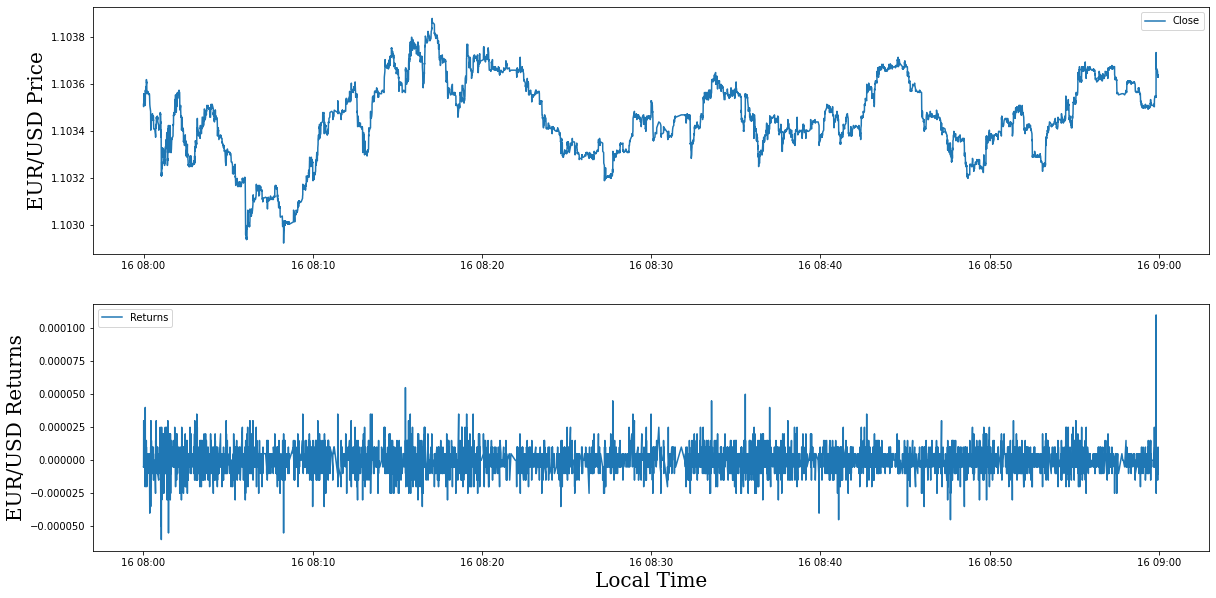
\includegraphics[width=\textwidth]{../plots/3__4__1__example_eur_usd.png}}
	\\
	\subfloat[Example of EUR / USD Daily Close Data, 1999 - 2020\label{fig:3__4__1__example_eur_usd_daily}]{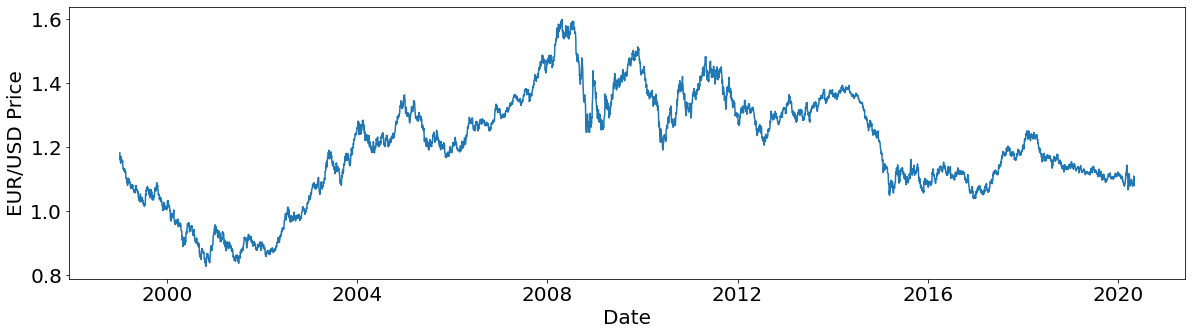
\includegraphics[width=\textwidth]{../plots/3__4__1__example_eur_usd_daily.png}}
	\label{fig:1__example_waveform_plots}
\end{figure}

\textbf{Quantisation}

The high frequency tick data that we obtain is often \textit{quantized}, and consists of only a few price levels. This is typical, as exchanges do not allow arbitrary prices to be transacted. In this case, the minimum price change possible is $5x10^-6 EUR/USD$. 

This is a violation of one of the core assumptions of the stochastic modelling: that the price levels are continuous. As the minimum return ($5x10^-6$) is small compared to the standard deviation of the returns, we ignore this problem in the project. However, we note that this could be a problem in extremely high frequency trading, where the price does not fluctuate much, hence causing the minimum return to be significant compared to the standard deviation of returns. 


\end{document}